\chapter{Introducción específica} % Main chapter title

\label{Chapter2}

%----------------------------------------------------------------------------------------
%	SECTION 1
%----------------------------------------------------------------------------------------
Este capítulo trata sobre los recursos tecnológicos utilizados en el trabajo que fueron desarrollados por terceros.

% Descripción de las plataformas tecnológicas que sostienen al trabajo
\section{Tecnologías utilizadas}

% docker
\emph{Docker} es un software que permite el uso y creación de contenedores de Linux.
Un contenedor es una unidad que empaqueta el código de un programa junto con sus dependencias.
Para crear un contenedor, \emph{Docker} se vale de el concepto de imagen.
Las imágenes son entidades aisladas que corren como contenedores durante el tiempo de ejecución sobre el motor de \emph{Docker}.
Los contenedores son entonces, una abstracción de la capa de aplicación de los sistemas Linux, como se puede visualizar en la figura \ref{fig:ch2WhatContainer}.
Varios contenedores pueden correr en el mismo ordenador como procesos aislados en el espacio de usuario.
La principal diferencia con las máquinas virtuales, es que estas son una abstracción del hardware del ordenador, transformando una única computadora en varios servidores.
Los contenedores en cambio, utilizan el kernel del sistema operativo del ordenador físico, no se abstrae un kernel, solo el espacio de aplicación o usuario.

% docker files
\emph{Docker} puede ser utilizado para construir imágenes definidas por el usuario.
Un \emph{Dockerfile} es un documento de texto que contiene todos los comandos que un usuario utilizaría para ensamblar una imagen.
El programador puede crear automáticamente una serie de comandos en sucesión al ejecutar un único comando sobre el \emph{Dockerfile}. 

% docker compose
\emph{Docker Compose}, según se define en su documentación \citep{WEBSITE:WhatDockerCompose}, es una herramienta para definir y correr aplicaciones de \emph{Docker} de múltiples contenedores.
Permite utilizar un archivo \emph{YAML} para configurar los servicios de la aplicación.
Luego, se puede crear y comenzar todos los servicios de la configuración utilizando un único comando.

\begin{figure}[h]
	\centering
	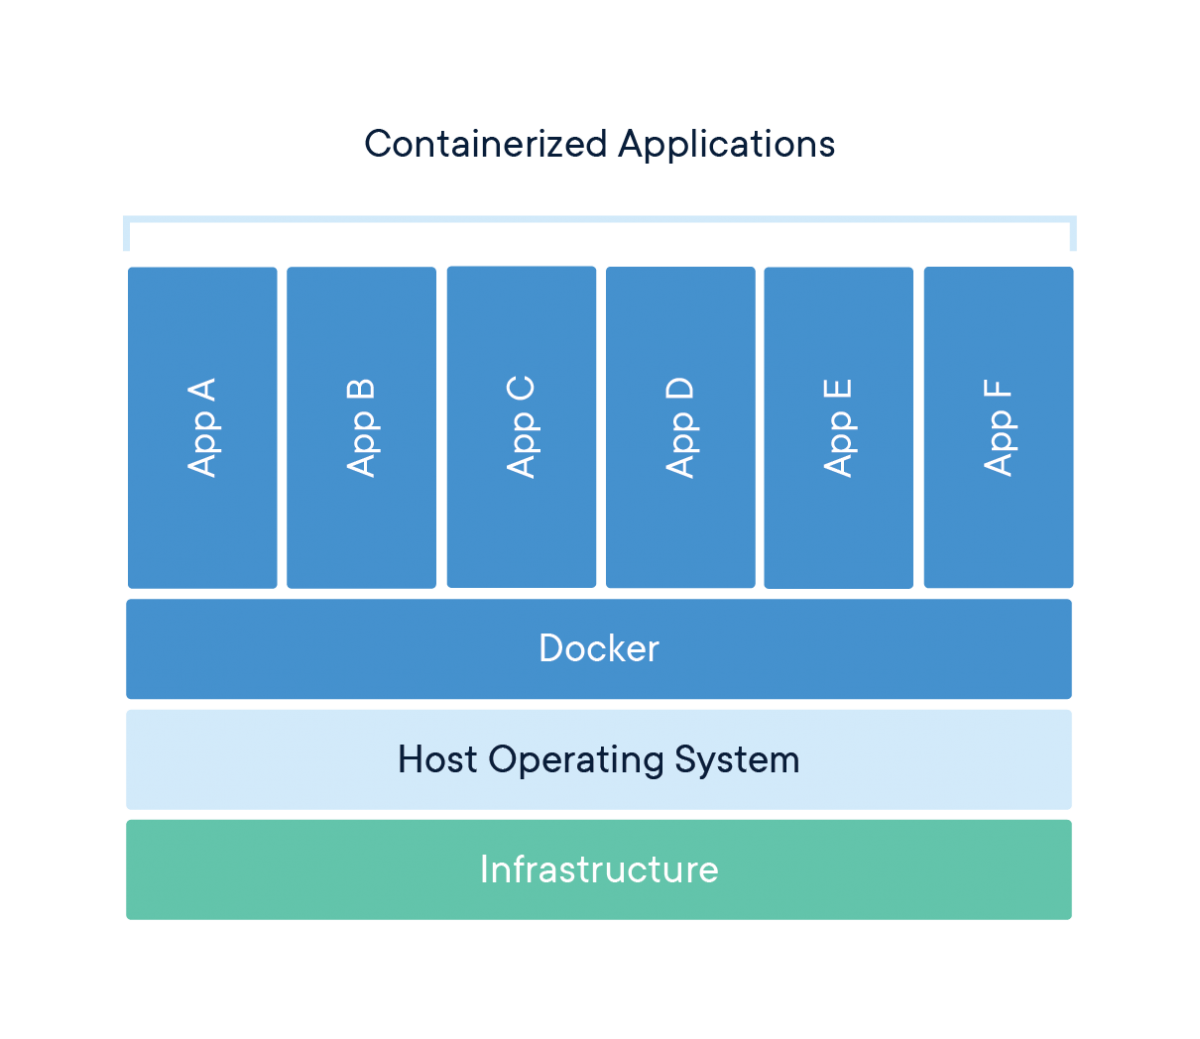
\includegraphics[width=\textwidth]{./Figures/ch2DockerContainer.png}
	\caption{Arquitectura de \emph{Docker}. \citep{WEBSITE:WhatContainer}}
	\label{fig:ch2WhatContainer}
\end{figure}

% nodejs
\emph{Nodejs} es un servidor asincrónico y orientado a eventos que ejecuta JavaScript.
Estas cualidades son una ventaja frente a las aplicaciones de concurrencia de múltiples hilos en el sistema operativo.
Ya que no se utilizan candados, no existe la posibilidad de bloquear el servidor.
Dado que fue diseñado para construir aplicaciones de red escalables, se eligió para formar parte del trabajo.

% python
\emph{Python} es un lenguaje de programación interpretado que tiene una gran cantidad de bibliotecas a disposición.
Muchas bibliotecas fueron útiles para desarrollar algunos servicios pequeños del proyecto.
Se utilizó para acelerar la creación de las partes más livianas del sistema.

% mosquitto
\emph{Eclipse Mosquitto} es un \emph{broker MQTT}.
Es liviano y puede ser ejecutado en ordenadores monoplaca.
Permite ser configurado con varios niveles de calidad de servicio, se pueden agregar usuarios con distintos permisos y es posible utilizar una capa de seguridad en los mensajes.
Uno de sus atractivos es la serie de programas utilitarios que incluye el proyecto y se integran en la terminal del sistema operativo.
Estas aplicaciones permiten realizar publicaciones y subscripciones para realizar pruebas, además se pueden crear contraseñas encriptadas para los usuarios.

% mongodb
"\emph{MongoDB} es una base de datos distribuida, basada en documentos y de uso general diseñada para desarrolladores de aplicaciones modernas y para la era de la nube". \citep{WEBSITE:MongoHome}
Se decidió utilizar esta tecnología para la capa de procesamiento debido a la afinidad que posee para realizar aplicaciones \emph{IoT}.
Además es la base de datos documental más utilizada actualmente \citep{WEBSITE:DBRanking} y se evaluó como aspecto relevante, ganar experiencia con esta tecnología.

% redis
	
% Descripción de las dependencias del trabajo
\section{Bibliotecas y paquetes de terceros}

% Angular & Angular Material

% express & cors

% mqtt & ws

% mongoose

% bcrypt & jsonwebtoken

% chai & mocha

% pyModbusTCP

% paho MQTT

% oitc/modbus-server

% Descripción del sistema marca Honeywell que funciona en planta.
\section{Sistema propietario del cliente}